% Created 2020-07-14 Tue 11:42
% Intended LaTeX compiler: pdflatex
\documentclass[presentation]{beamer}
\usepackage[utf8]{inputenc}
\usepackage[T1]{fontenc}
\usepackage{graphicx}
\usepackage{grffile}
\usepackage{longtable}
\usepackage{wrapfig}
\usepackage{rotating}
\usepackage[normalem]{ulem}
\usepackage{amsmath}
\usepackage{textcomp}
\usepackage{amssymb}
\usepackage{capt-of}
\usepackage{hyperref}
\usetheme{UoB}
\author{Mark Blyth}
\date{\textit{[2020-07-15 Wed]}}
\title{Bayesian methods for the control-based continuation of multiple-timescale systems}
\hypersetup{
 pdfauthor={Mark Blyth},
 pdftitle={Bayesian methods for the control-based continuation of multiple-timescale systems},
 pdfkeywords={},
 pdfsubject={},
 pdfcreator={Emacs 26.3 (Org mode 9.1.9)}, 
 pdflang={English}}
\begin{document}

\maketitle

\section{Intro}
\label{sec:orgfd158cb}
\begin{frame}[label={sec:org4db2d50}]{Plan de jour}
\begin{itemize}
\item CBC maths
\item Surrogate modelling
\item Novel discretisations
\end{itemize}
\end{frame}
\begin{frame}[label={sec:orga1cbe38}]{Plan de jour}
\begin{itemize}
\item \alert{CBC maths}
\item Surrogate modelling
\item Novel discretisations
\end{itemize}
\end{frame}
\section{CBC background}
\label{sec:org0af6836}
\begin{frame}[label={sec:org33938b2}]{What is CBC?}
Dynamics are `what something does'

\begin{center}
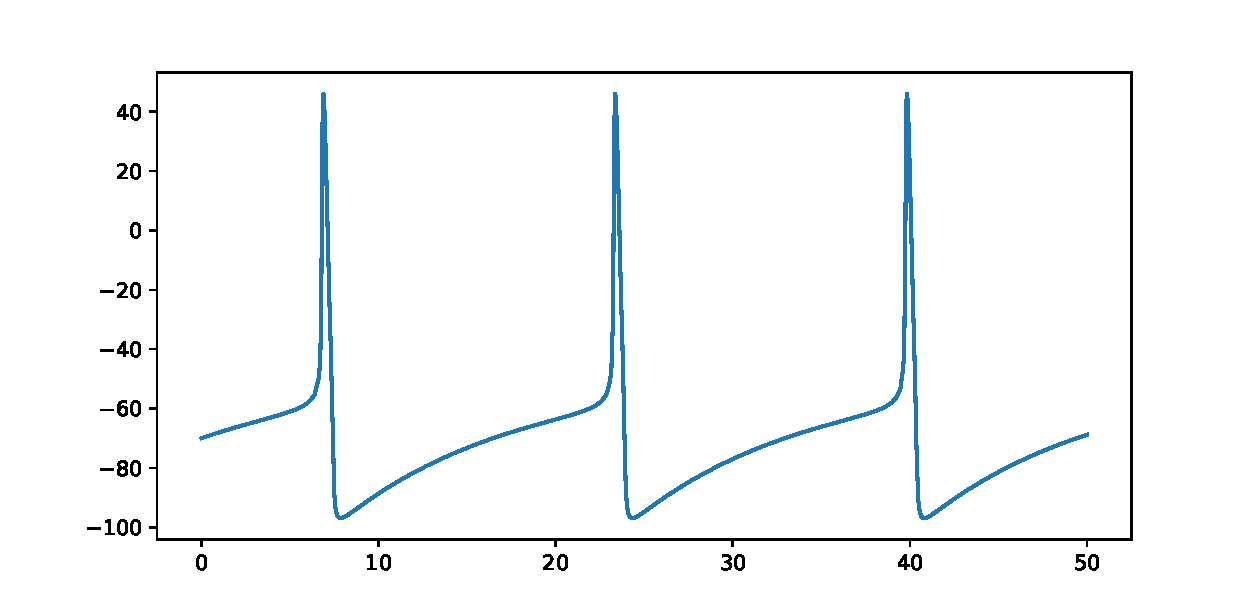
\includegraphics[width=.9\linewidth]{./HH.pdf}
\end{center}
\end{frame}

\begin{frame}[label={sec:org273aa8e}]{What is CBC?}
\begin{center}
A bifurcation is a change in dynamics
\end{center}
\begin{columns}
\begin{column}{0.5\columnwidth}
\begin{center}
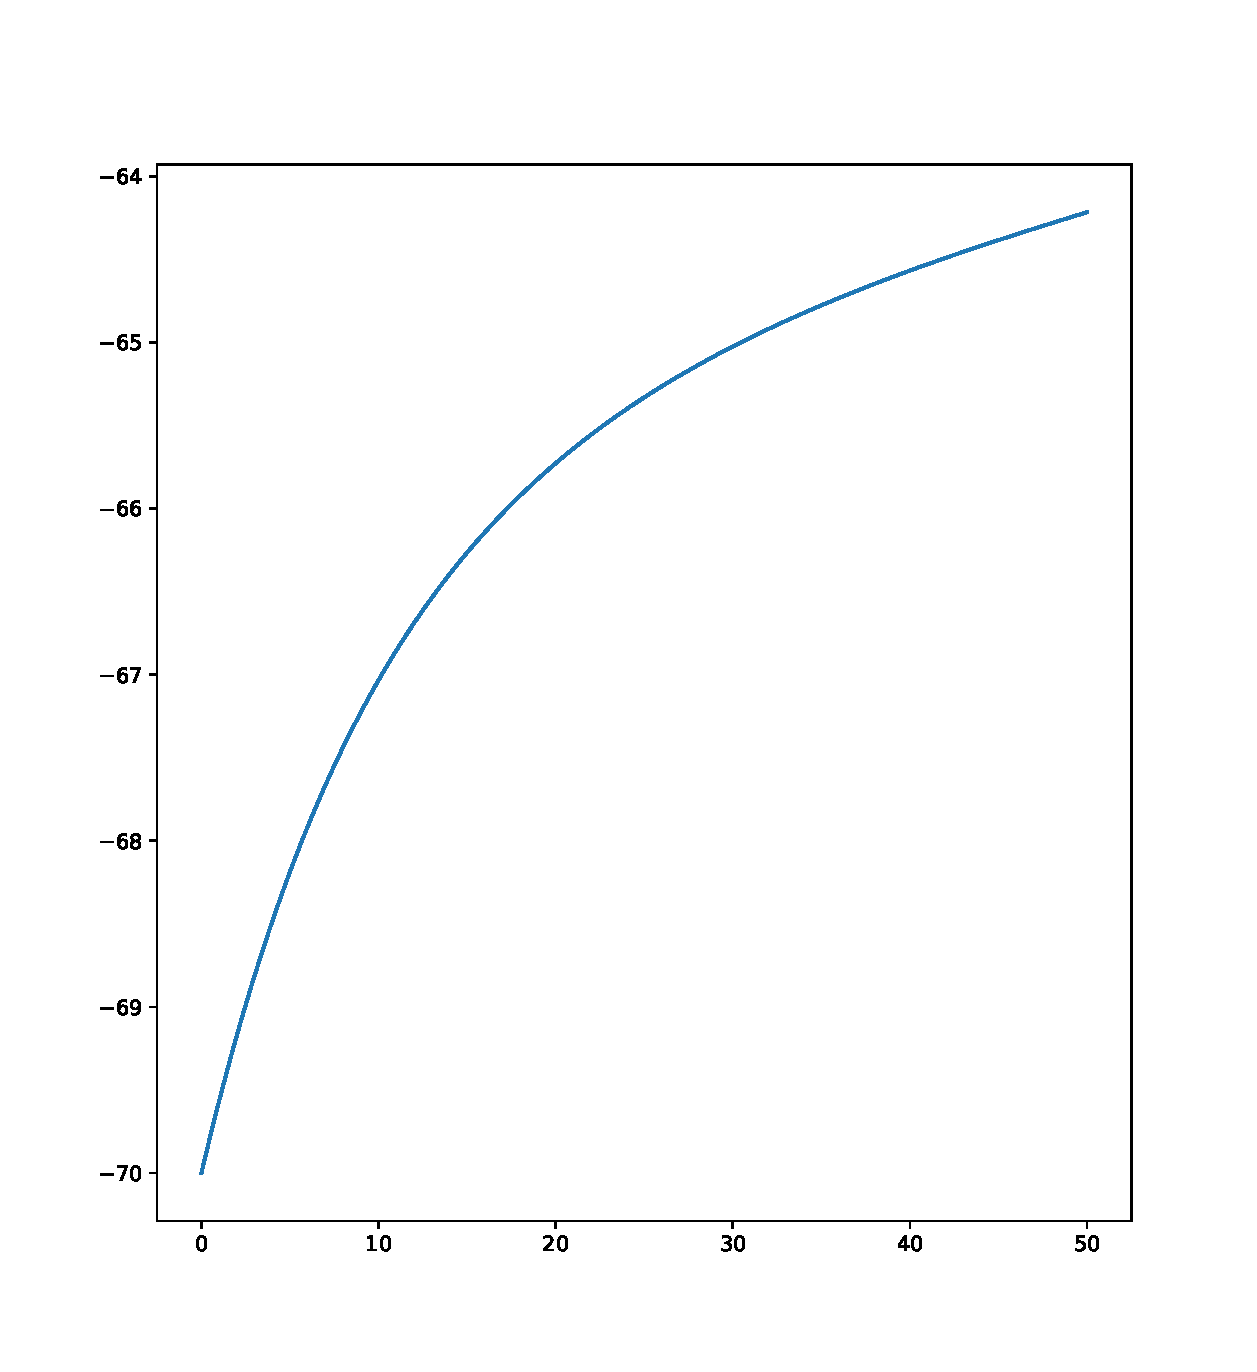
\includegraphics[height=.8\textheight]{./excitable.pdf}
\end{center}
\end{column}

\begin{column}{0.5\columnwidth}
\begin{center}
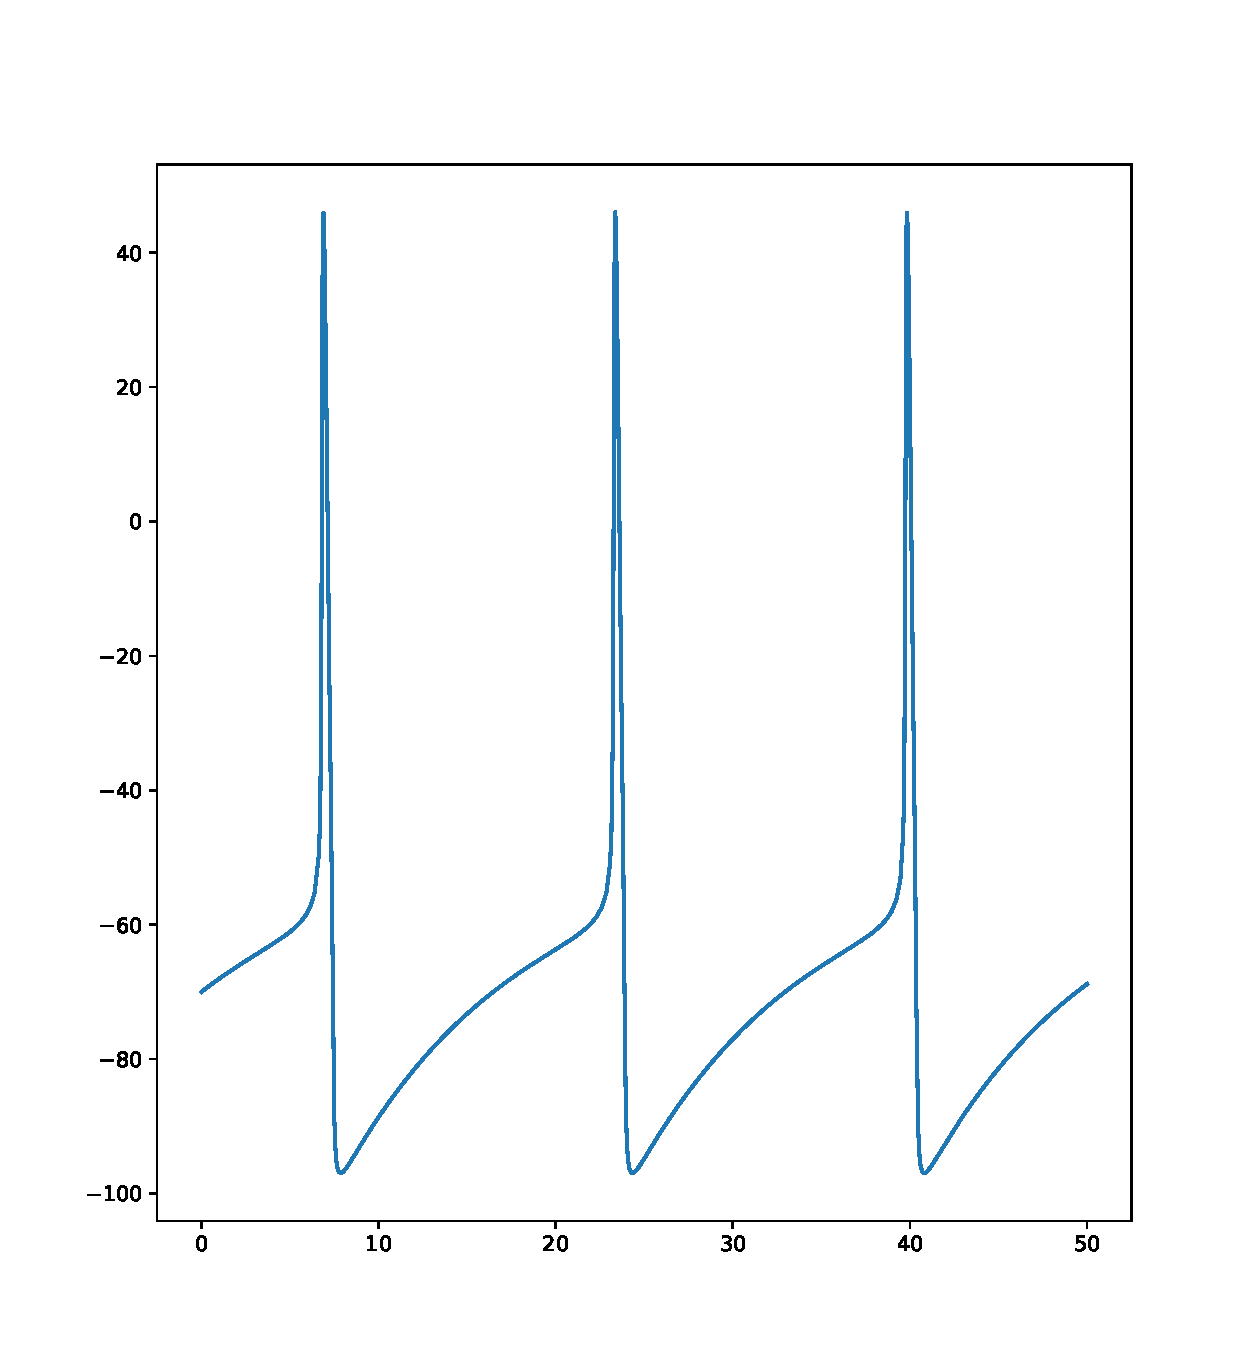
\includegraphics[height=.8\textheight]{./spiking.pdf}
\end{center}
\end{column}
\end{columns}
\end{frame}

\begin{frame}[label={sec:org7746c9d}]{What is CBC?}
Bifurcation analysis:
\begin{enumerate}[<+->]
\item Find a feature
\begin{itemize}
\item Eg. a rest-state or sustained oscillation
\end{itemize}
\item Change a parameter slightly
\begin{itemize}
\item Eg. inject more current in a neuron
\end{itemize}
\item Find where the feature moved to
\begin{itemize}
\item Eg. increase in rest-state membrane potential
\end{itemize}
\item Bifurcations occur when features change, appear, or disappear
\end{enumerate}
\end{frame}

\begin{frame}[label={sec:org0cdda59}]{What is CBC?}
\begin{itemize}
\item Numerical continuation:
\begin{itemize}
\item Features \(x\) defined given by \(f(x, \lambda)=0\)
\item Change \(\lambda\), see how \(x\) changes
\end{itemize}
\end{itemize}

\vfill

\begin{block}{George Box}
All models are wrong, but some are useful
\end{block}
\end{frame}

\begin{frame}[label={sec:org8772d36}]{What is CBC?}
Control-based continuation; model-free bifurcation analysis:
\begin{enumerate}[<+->]
\item Build a system controller
\begin{itemize}
\item Put in target \(u^*(t)\)
\item Controller makes system follow \(u^*(t)\)
\end{itemize}
\item Find noninvasive \(u^*(t)\)
\begin{itemize}
\item Noninvasiveness = no control action applied
\item No control action = system behaves naturally
\end{itemize}
\item Change a parameter
\item Find how noninvasive \(u^*(t)\) changed
\begin{itemize}
\item Tracks system features, bifurcations without ever needing a model
\end{itemize}
\end{enumerate}
\end{frame}
\begin{frame}[label={sec:orgfc8154a}]{CBC}
\begin{block}{Control-based continuation}
A model-free bifurcation analysis method. Uses a controller to stabilise a system, and continuation to track features.
\end{block}

\vfill
My project: use CBC to analyse the bifurcations that make neurons fire
\end{frame}

\section{Discretisation}
\label{sec:org3734515}
\begin{frame}[label={sec:orgcadc1ae}]{What is discretisation?}
\begin{itemize}[<+->]
\item Periodic orbits are functions satisfying \(f(t) = f(t+T)\)
\item Tracking these means solving the functional equation \(I\left[u^*\right] = \int_0^T\left[u(u^*, t)\right]^2\mathrm{d}t = 0\) for function \(u^*(t)\)
\begin{itemize}
\item This is hard!
\item \emph{[interesting aside: optimal control developed some nice approaches for solving variational equations]}
\end{itemize}
\item Discretisation lets us solve the problem by solving a finite set of equations
\end{itemize}
\end{frame}

\begin{frame}[label={sec:orgec67196}]{What is discretisation?}
Goal: solve \(I\left[u^*\right] = 0\)
\begin{enumerate}
\item Translate problem to system of vector-valued equations
\item Solve system numerically
\item Translate solution back to a continuous function
\end{enumerate}

\vfill
Translation between continuous and vector-valued systems is discretisation
\end{frame}

\begin{frame}[label={sec:orgce31744}]{What is discretisation?}
\begin{definition}[Discretisation]
The act of representing a continuous signal by a discrete counterpart
\end{definition}

\vfill
We want a discretisation that
\begin{itemize}
\item Has minimal discretisation error
\item Is low-dimensional
\end{itemize}
\end{frame}

\begin{frame}[label={sec:org07ddedd}]{How do we discretise?}
\begin{itemize}[<+->]
\item Let \(\mathbf{u^*}\) be some vector `representing' the signal \(u^*(t)\)
\begin{itemize}
\item Eg. Fourier: let our periodic target be \(u^*(t) = a_0 + \sum a_i \cos i\omega t + \sum b_i \sin i\omega t\)
\end{itemize}
\item We can represent the signal by its Fourier harmonics \(\mathbf{u^*}=\{a_0, a_i, b_i\}\)
\item \(u^*(t)\) can be represented by \(\mathbf{u}^*\) with minimal error
\begin{itemize}
\item \(\mathbf{u^*}\) is a discretisation
\item Represents a continuous function as finite-dimensional vector, with minimal error
\end{itemize}
\item The functional problem can be rewritten as \(I\left(\mathbf{u}^*\right)=0\)
\begin{itemize}
\item Finite-vector equation, solvable!
\end{itemize}
\end{itemize}
\end{frame}

\begin{frame}[label={sec:org49b70ba}]{Issues with discretisation}
\begin{itemize}
\item Solving the discretised system takes a long time when it is high-dimensional
\vfill
\item Neuron signals require lots of Fourier harmonics to discretise
\vfill
\item Higher-order harmonics are harder to get \emph{[Nyquist cap]} and less accurate \emph{[SNR]}
\end{itemize}
\end{frame}

\begin{frame}[label={sec:orgeab5ee7}]{Plan de jour}
\begin{itemize}
\item CBC maths
\item \alert{Surrogate modelling}
\item Novel discretisations
\end{itemize}
\end{frame}
\section{The need for surrogates}
\label{sec:org5d1755d}
\begin{frame}[<+->][label={sec:orgc59d2a6}]{The need for surrogates}
\begin{itemize}
\item Recent work: local surrogate models for experimental data
\end{itemize}

\vfill

\begin{definition}[Surrogate models]
A local model for data, that can be used in place of experimental recordings
\end{definition}

\vfill

\begin{itemize}
\item Record experimental data
\item Fit a surrogate model
\item Perform analysis, eg. discretisation, on model instead of data
\end{itemize}
\end{frame}

\begin{frame}[label={sec:org23fc629}]{Why surrogates?}
Real data are noisy
\begin{center}
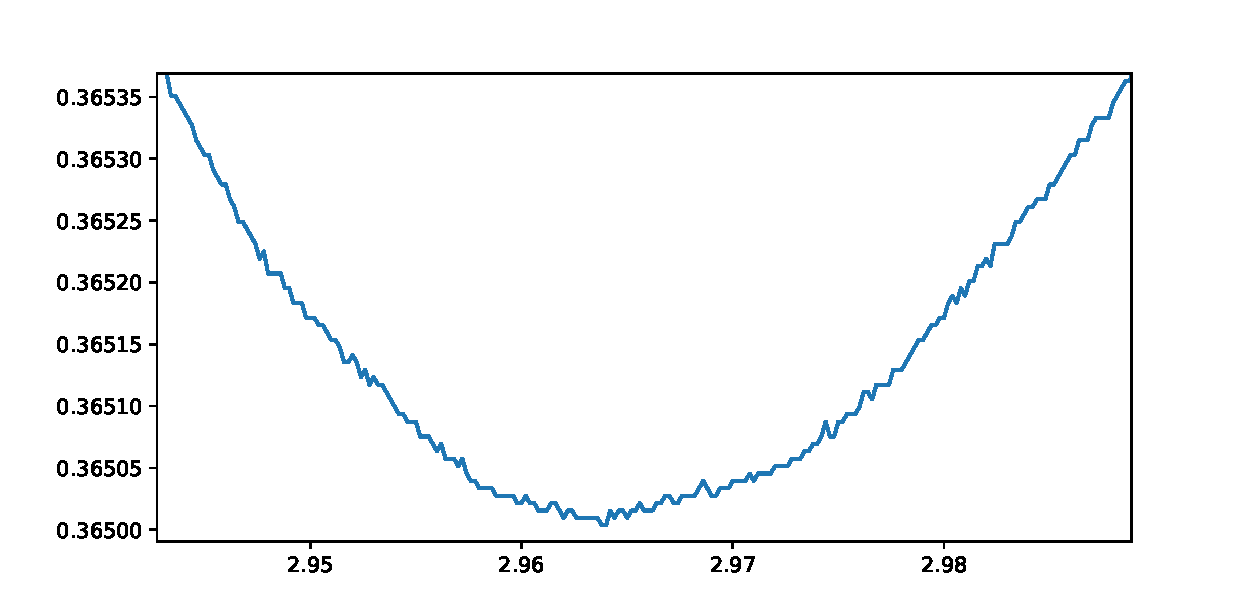
\includegraphics[width=.9\linewidth]{./noisy.pdf}
\end{center}

\begin{center}
\emph{[Thanks to LR for the data]}
\end{center}
\end{frame}

\begin{frame}[label={sec:orgc50c0c5}]{Why surrogates?}
Real data are `fast'
\begin{center}
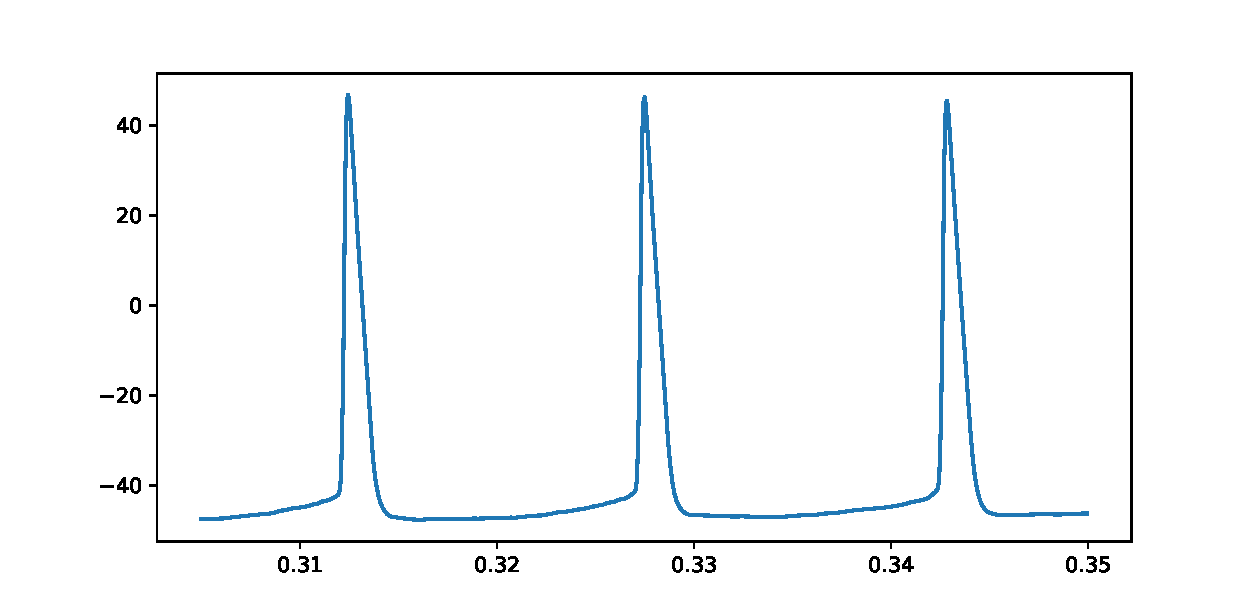
\includegraphics[width=.9\linewidth]{./fast.pdf}
\end{center}

\begin{center}
\emph{[Thanks to KTA for the data]}
\end{center}
\end{frame}

\begin{frame}[<+->][label={sec:org4ef586f}]{Why surrogates?}
\begin{itemize}
\item We want to get rid of noise to get the best possible discretisation
\begin{itemize}
\item Fourier should encode only signal, not signal + noise
\end{itemize}
\end{itemize}
\vfill
\begin{itemize}
\item Fast signals mean lots of high-frequency energy
\begin{itemize}
\item High signal-to-noise ratio on the harmonics that give sharp spikes
\item Simple low-pass filters would remove both noise \emph{and} signal
\end{itemize}
\end{itemize}
\vfill
\begin{itemize}
\item A good surrogate lets us remove noise in a statistically optimal way
\begin{itemize}
\item Less noise = better discretisation
\end{itemize}
\end{itemize}
\end{frame}

\section{Bayes}
\label{sec:org261c9cf}
\begin{frame}[label={sec:org60a294a}]{A primer on Bayes}
The laws of probability, applied to beliefs instead of proportions-of-outcomes
\vfill
\begin{itemize}
\item \emph{[Frequentist]} probability:
\begin{itemize}
\item How likely is something to happen?
\item An event is known to happen some proportion of the time; how can I reason about its outcomes?
\end{itemize}
\end{itemize}
\vfill
\begin{itemize}
\item \emph{[Bayesian]} beliefs:
\begin{itemize}
\item Encoding uncertain beliefs; reasoning in the face of ignorance
\item I have some beliefs about an event; how can I update my beliefs after seeing some evidence?
\item Let's us combine beliefs and evidence to make better decisions
\end{itemize}
\end{itemize}
\end{frame}

\begin{frame}[<+->][label={sec:orgf423900}]{Bayesian surrogates}
\begin{itemize}
\item We have a `true' signal \(f(t)\), but we can only see noise-corrupted samples \(y_i = f(t_i) + \varepsilon\)
\begin{itemize}
\item \(f(t)\) is unknown, but we can reason about it with Bayes
\end{itemize}
\item Prior: assume \(\varepsilon\sim\mathcal{N}(0, \sigma^2)\)
\begin{itemize}
\item Single observation: \(y_i \sim \mathcal{N}(f(t_i), \sigma_n^2)\)
\item All observations: \(\mathbf{y} \sim \mathcal{N}(f(\mathbf{t}), \Sigma_n^2)\)
\end{itemize}
\item Let's estimate \(y^*=f(t^*)\) at unseen data \(t^*\)
\begin{itemize}
\item Joint distribution: \(p(f(t^*),t^*,y,t) \sim \mathcal{N}(\mu, \Sigma_k^2)\)
\item Conditional distribution: \(p(f(t^*)|t^*, y, t)\)
\end{itemize}
\item This is Gaussian process regression!
\end{itemize}
\end{frame}

\begin{frame}[label={sec:org28f4d36}]{Gaussian process regression surrogates}
Build a statistically optimal regression model from noisy observations

\begin{center}
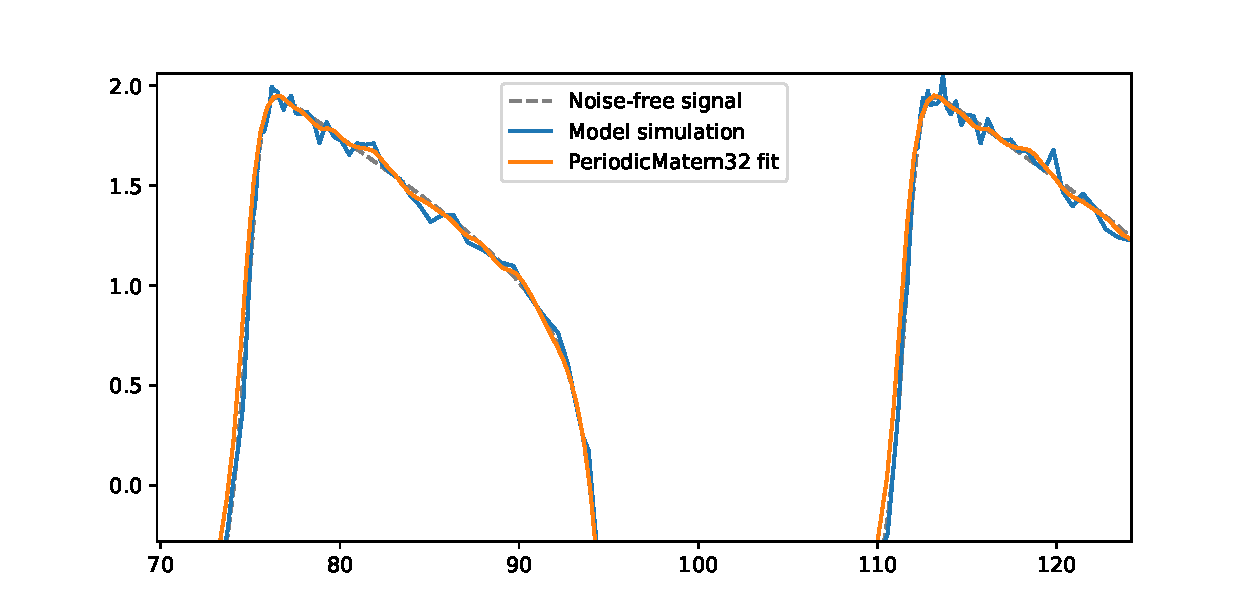
\includegraphics[width=.9\linewidth]{./matern.pdf}
\end{center}
\end{frame}

\begin{frame}[<+->][label={sec:org9950fb4}]{GPR results}
\begin{itemize}
\item GPR is Bayesian
\begin{itemize}
\item Covariance function specifies our initial belief about the data
\item Conditioning step updates this belief after seeing data
\end{itemize}
\item Covariance functions generally assume stationarity
\begin{itemize}
\item Assume smooth, nice signals
\item Neuron data are highly non-stationary
\end{itemize}
\item Stationary covariance = poorly encoded beliefs = low belief in posterior
\begin{itemize}
\item Bayes with bad priors = bad results!
\end{itemize}
\end{itemize}
\end{frame}

\begin{frame}[label={sec:org6c1e45c}]{GPR results}
\begin{center}
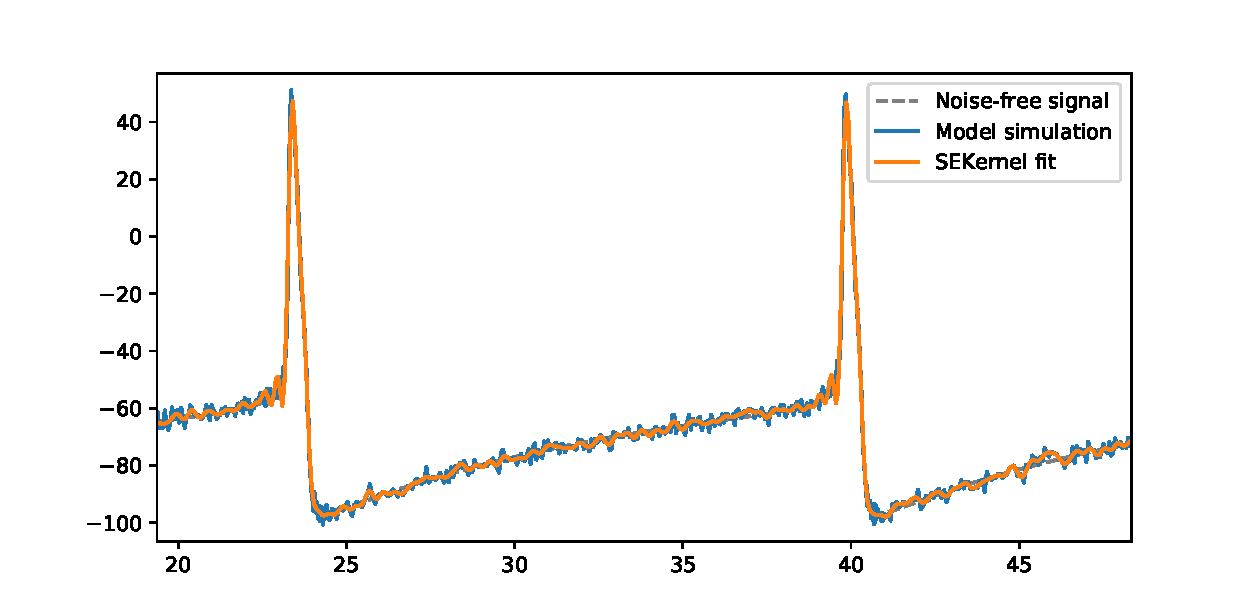
\includegraphics[width=.9\linewidth]{./badfit.pdf}
\end{center}
\end{frame}

\begin{frame}[label={sec:org555f6e7}]{GPR results}
\begin{center}
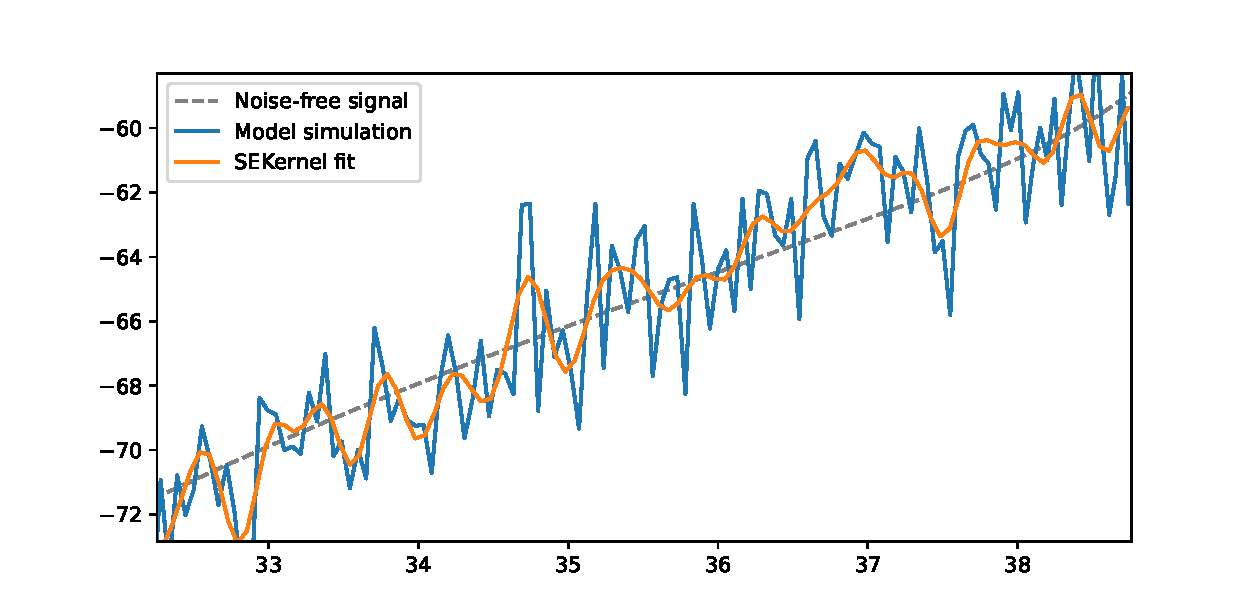
\includegraphics[width=.9\linewidth]{./badfit2.pdf}
\end{center}
\end{frame}

\begin{frame}[<+->][label={sec:org97e1898}]{GPR results}
\begin{itemize}
\item Stationary GPR, non-stationary data = overly flexible models
\begin{itemize}
\item Needs to change rapidly to accomodate spikes
\item Stationary = equally flexible everywhere, even away from spikes
\item Overfit noise, instead of averaging it out
\end{itemize}
\item Non-stationary would fix this
\begin{itemize}
\item Flexible near spikes
\item Inflexible away from them
\item Smooths out noise, while also modelling spikes
\end{itemize}
\item Non-stationary GPR is hard!
\end{itemize}
\end{frame}
\section{Splines}
\label{sec:orgd0a1eef}
\begin{frame}[<+->][label={sec:org3dd9004}]{Splines}
\begin{itemize}
\item Less flexible alternative: splines
\item Choose some representative points
\item Place a piece of cubic polynomial between each point
\item Choose polynomials so that the function is smooth
\item Finite, low degree-of-freedom, forcibly averages out noise
\end{itemize}
\end{frame}
\begin{frame}[<+->][label={sec:orgfdcbf8e}]{Bayesian splines}
\begin{itemize}
\item Choosing representative points is hard
\item Alternative: don't!
\begin{itemize}
\item Let \(\xi\) be a vector of representative points
\item Find \(p(\xi|x,y)\)
\item Use that to estimate \(p(f | \xi, x, y)\)
\end{itemize}
\item This is Bayesian free-knot splines
\end{itemize}
\end{frame}
\begin{frame}[label={sec:org57131c4}]{Splines as a surrogate}
Result 1: splines outperform stationary GPR as neuronal data surrogate

\begin{center}
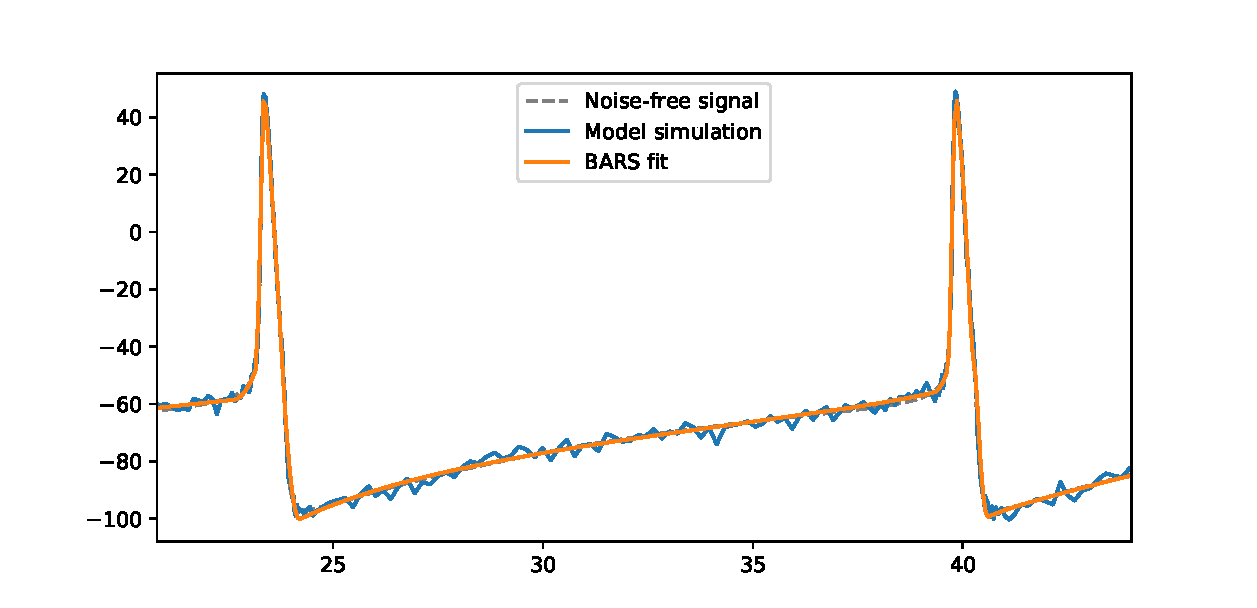
\includegraphics[width=.9\linewidth]{./bars.pdf}
\end{center}
\end{frame}

\section{Discretisation}
\label{sec:orgf5a35dd}
\begin{frame}[label={sec:org19637e9}]{Plan de jour}
\begin{itemize}
\item CBC maths
\item Surrogate modelling
\item \alert{Novel discretisations}
\end{itemize}
\end{frame}
\begin{frame}[<+->][label={sec:orgb7b6318}]{The issue with surrogates}
My current work\ldots{}
\begin{itemize}
\item Bayesian free-knot splines gives a good noise-free surrogate model
\begin{itemize}
\item Can apply Fourier discretisation on the surrogate
\item Can get arbitrarily many mostly-accurate Fourier coefficients
\end{itemize}
\item Issue: too many coefficients are needed to discretise the signal
\begin{itemize}
\item Too many = slow, inaccurate CBC
\item \emph{Question: how many do we actually need?}
\end{itemize}
\item We can reconstruct signal from splines models
\begin{itemize}
\item Is this a discretisation?
\end{itemize}
\end{itemize}
\end{frame}

\begin{frame}[<+->][label={sec:org3f0c9d7}]{Splines as a discretisation}
\begin{itemize}
\item Splines models are of form \(\hat{f}(x) = \sum \beta_i b_i(x)\)
\begin{itemize}
\item \(b_i(x)\) form a set of basis functions over splines models
\end{itemize}
\item For a basis set \(b_i\), can the associated \(\beta_i\) discretise a signal?
\begin{itemize}
\item Result 2: probably\ldots{}
\item This is my current work
\end{itemize}
\end{itemize}
\end{frame}

\begin{frame}[label={sec:orgdb53b41}]{Spline discretisation}
8-dimensional discretisation; but does it work with continuation?
\begin{center}
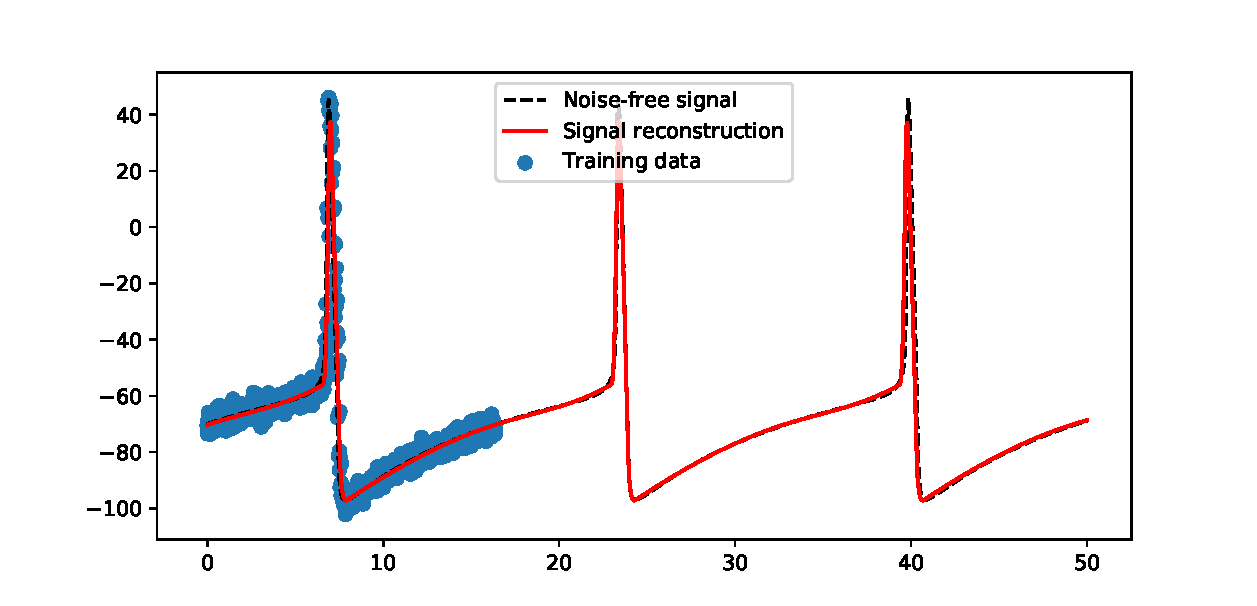
\includegraphics[width=.9\linewidth]{./HHdisc.pdf}
\end{center}
\end{frame}
\section{Outro}
\label{sec:orgfdebd32}
\begin{frame}[label={sec:orgfcc8af7}]{Where next?}
\begin{itemize}
\item Compare Fourier vs splines discretisation
\begin{itemize}
\item What error for what discretisation-size?
\end{itemize}
\item See if the discretisation breaks down with stochastic models
\begin{itemize}
\item It probably will
\end{itemize}
\item Test the discretisation with continuation
\end{itemize}
\end{frame}
\end{document}
